% ---------------------------------------------------------------------------
% Calibration, results, relaxation, discussion, conclusion (input for theory_section.tex)
% Numbers come from manuscript/numbers.tex (generated by scripts/06_summary.py)
% ---------------------------------------------------------------------------
\section{Calibration on the data without dissipation}
\label{sec:calib}
The simulation starts at $t=1$~s from a Bose distribution with the measured
$N=5.6\times10^4$ and $T=240$~nK and no condensate, and is run to $t=2$~s with
the frequency ramp of Fig.~S1 of Ref.~\cite{MelladoMunoz2020}. Three
parameters are adjusted on $N(t)$, $T(t)$ and $F(t)$ of the data without K
(blue symbols of Fig.~2 of Ref.~\cite{MelladoMunoz2020}, 30 points): the
trap depth at $t=1$~s, $\eta_1=U_t/k_BT_1=\etaone$, its exponent $p=\pexp$,
and a background loss rate $\gamma_{\rm bg}=\gbg$~s$^{-1}$. The scale of the
trap frequency is not free: with $s_\omega=0.85$ the best fit is worse by a
factor of three in $\chi^2$ than with $s_\omega=1$, so the frequency
calibrated from Eq.~(1) in Ref.~\cite{MelladoMunoz2020} is also the one that
describes the kinetics, and we keep $s_\omega=1$. With these values the model
reproduces $N(t)$ to \ndNrms\% rms, $F(t)$ to \ndFrms{} rms and $T(t)$ to
\ndTrms\% rms, the temperature being systematically low in the middle of the
ramp [Fig.~\ref{fig:ramp}]. Two remarks on this calibration are needed before
the data with K are discussed. First, the fitted $\eta_1$ is small: the trap is
only $3$ to $6$ thermal energies deep, so the evaporation is fast and the
thermal cloud follows the trap depth quasi-statically; this is the regime in
which the gas is most sensitive to anything that changes the rate at which
energy is removed. Second, the background loss needed to reproduce $N(t)$ is
larger than a vacuum lifetime would give; it absorbs the loss channels not in
the model (evaporation along the direction of gravity, spilling by
anharmonicity), and it is energy-neutral by construction, so it does not
change the conclusions below, which concern the temperature and the
condensed fraction.

\section{Dissipative distillation}
\label{sec:diss}
The K atoms enter the model only through $\gamma_K(t)$. The rate measured in
Fig.~1(b) of Ref.~\cite{MelladoMunoz2020}, $\gamma_K=0.112\,t$~Hz, under-predicts
the loss actually present in the Fig.~2 data: the ratio $N_{\rm K}/N_{\rm no\,K}$
of the measured atom numbers falls as $\exp(-ct^3/3)$ with $c=0.18$~Hz\,s$^{-2}$
(and $c=0.46$~Hz\,s$^{-2}$ for the data at four times the K density), i.e. as
if $\gamma_K\propto t^2$ with an integrated loss $1.8$ times (1.2 times) the
measured one at $t=2$~s. We have not identified the origin of this difference
and use both laws; the conclusions do not depend on the choice, and the
figures show the empirical law. With this single input, the model reproduces
the atom number [\dsNrms\% rms, $N(2\,{\rm s})=\dsNmod\times10^3$ against
$\dsNdat\times10^3$] and the condensed fraction [\dsFrms{} rms,
$F(2\,{\rm s})=\dsFmod$ against $\dsFdat$] of the distillation data, and for
the four-fold dissipation $F(2\,{\rm s})=\dqFmod$ against $\dqFdat$
[Fig.~\ref{fig:ramp}, Fig.~\ref{fig:ramp4}]. It does not reproduce the
temperature. In the model the temperature of the gas with K is the same as
without K to within 2\% at all times, as expected for a loss that is uniform
in energy. The data separate after $t\simeq1.5$~s: at $t=2$~s the model gives
$\dsTmod$~nK against the measured $\dsTdat$~nK with K (\dqTmod{} against
\dqTdat~nK at four times the K density), whereas without K it gives
$\ndTmod$ against $\ndTdat$~nK; the rms deviations over the ramp are
\dsTrms\%, \dqTrms\% and \ndTrms\% respectively. The thermal cloud of the model
is at or above saturation throughout the ramp, $\mu_{\rm th}\ge\mu_c$
[Fig.~\ref{fig:ramp}(d)], because the condensate grows more slowly than the
evaporation lowers the saturated number: the model is on the ``undercritical''
side of the equilibrium curve, $F<F_{\rm eq}$, with and without K
[Fig.~\ref{fig:phase}], and the two trajectories in the $F$-$\tau$ plane
differ only by the shift of $\tau$ that comes from the lower $N$. The
measured trajectory with K, which rises at $\tau\simeq1$ with
$\mu_{\rm th}<0$, has no counterpart in the model.

The reason is quantitative and does not depend on the details of the
evaporation. A thermal cloud of $6.8\times10^3$ atoms at $76$~nK in the
end-of-ramp trap, the state measured at $t=2$~s with K, is undersaturated by
26\%; the kinetic equations fill it from the condensate with the collision
integral $I_{12}$ at a rate set by the Rb-Rb cross section and the thermal
density, and the condensed fraction falls from 0.46 to 0.38 with a $1/e$ time
of 50~ms, while the temperature drops from 79 to 64~nK because the atoms
leaving the condensate have to be raised to the thermal energy
[Sec.~\ref{app:uniform}]. Started from the state measured at the beginning of
the hold of Fig.~4 (15\% undersaturated), the model restores
$\mu_{\rm th}=\mu_c$ within the same 50~ms. The relaxation time measured in
Ref.~\cite{MelladoMunoz2020} is $3.9$~s, a factor of 80 longer. The benchmark
of Sec.~\ref{sec:model} puts the uncertainty of $I_{12}$ at a factor of two
to four; the elastic collision rates of 10 to 65~Hz quoted in
Ref.~\cite{MelladoMunoz2020} give the same scale. We therefore conclude that
the ergodic kinetic theory excludes a supercritical state of the kind defined
by the measured $(N,T,F)$, if $T$ is the temperature of the thermal cloud in
the sense of the kinetic theory (a Bose distribution of the energies above
$\mu_c$).

\section{Relaxation after the dissipation is switched off}
\label{sec:hold}
For the hold of Fig.~4 and Fig.~S2(ii) the trap is frozen at the end of a
different ramp, so it is calibrated again on the hold data without K
($\eta_{\rm hold}=\etahold$ at the initial temperature, frequency scale
$\somhold$ relative to the 99~Hz calibrated in Ref.~\cite{MelladoMunoz2020},
$\gamma_{\rm bg}=\gbghold$~s$^{-1}$), and the hold with K is then predicted
from its measured initial state. The condensed fraction is reproduced in both
series [Fig.~\ref{fig:hold}]: with K it rises from $\hdsFzero$ to $\hdsFend$ in
4~s in the model against $0.18$ to $0.57$ in the data, and without K from
$\hndFzero$ to $\hndFend$ against $0.20$ to $0.75$ (last point at 2.5~s). The model temperature
falls faster than the measured one (to $\hdsTend$~nK against $63$~nK), so the
model stays below the measured $\tau$ by $0.1$ to $0.2$. Evaluated with the
same formula as in Ref.~\cite{MelladoMunoz2020}, the model's excess fraction
$\delta F=F-F_{\rm eq}(\tau)$ is $\hdsdFmid$ at $1.5$~s and $\hdsdFend$ at
4~s, against the measured $0.28$ and $0.13$: the model has a positive $\delta F$ that grows slowly and reaches the
late-time value of the data, but it shows neither the maximum nor the decay. The positive $\delta F$ of the model is not a
supercritical state: $\mu_{\rm th}>\mu_c$ throughout, and $F$ is within
$0.02$ of the fraction the gas would have in equilibrium at the same number
and energy ($F_{N,E}$, dash-dotted lines in Fig.~\ref{fig:hold}). It
reflects the difference between an equilibrium at fixed $(N,E)$ and the
constant-temperature curve $F_{\rm eq}(\tau)$ for a gas that is still
evaporating, together with the systematic offset between the kinetic
temperature and the Gaussian-fit temperature discussed in
Sec.~\ref{sec:model}. Section~\ref{sec:NE} applies the same comparison to
the data themselves.

\section{Equilibrium at fixed number and energy}
\label{sec:NE}
The excess fraction $\delta F$ of Ref.~\cite{MelladoMunoz2020} is defined
relative to $F_{\rm eq}(\tau)$ at the measured temperature, that is,
relative to the state the gas would reach in contact with a bath at that
temperature. A trapped gas has no such bath. Once the K atoms are removed,
its only exchanges with the outside are the loss of atoms and the
evaporation over the barrier, and both are slow at fixed trap depth. The
state it can actually reach is the equilibrium at its own atom number and
energy, and the kinetic models of Secs.~\ref{sec:hold} and
\ref{sec:phasespace} reach it in $0.05$ to $0.2$~s. We therefore compute
this reference directly from the data. Here, $E$ is the energy of the
measured state: that of an ideal Bose gas with the fugacity $z$ that gives
the measured thermal number at the measured temperature ($z=0.67$ to $1$),
plus the Thomas-Fermi energy $\frac57\mu_cN_c$ of the condensate; $T'$ is
the temperature at which a saturated cloud and a condensate have the same
$N$ and $E$, with the condensed fraction $F_{N,E}=F_{\rm eq}(T'/T_c)$ from
Eq.~(1) of Ref.~\cite{MelladoMunoz2020}, and the calibrated trap frequency
is used throughout. Figure~\ref{fig:NE} shows the result for the three
series with K-induced loss or a hold, and Table~\ref{tab:NE} the averages.

\begin{table}[t]
\caption{Measured condensed fraction minus the equilibrium value at the
measured temperature [Eq.~(1), the reference of
Ref.~\cite{MelladoMunoz2020}] and minus the equilibrium value at the
measured number and energy, averaged over the digitized points of each
series (mean $\pm$ r.m.s.\ scatter). The last column is the range of the
ratio between the measured temperature and the temperature of the
fixed-$(N,E)$ equilibrium [DATA, scripts/15].}
\label{tab:NE}
\begin{ruledtabular}
\begin{tabular}{lcccc}
series & points & $F-F_{\rm eq}(T)$ & $F-F_{N,E}$ & $T/T'$ \\
\hline
with K, ramp $t\ge1.5$~s & 6 & $0.29\pm0.08$ & $0.09\pm0.02$ & $1.07$--$1.17$ \\
with K, hold $0$--$4$~s & 12 & $0.29\pm0.10$ & $0.10\pm0.03$ & $1.08$--$1.23$ \\
without K, hold $0$--$2.5$~s & 9 & $0.09\pm0.07$ & $0.03\pm0.03$ & $0.98$--$1.09$ \\
\end{tabular}
\end{ruledtabular}
\end{table}

\begin{figure}[t]
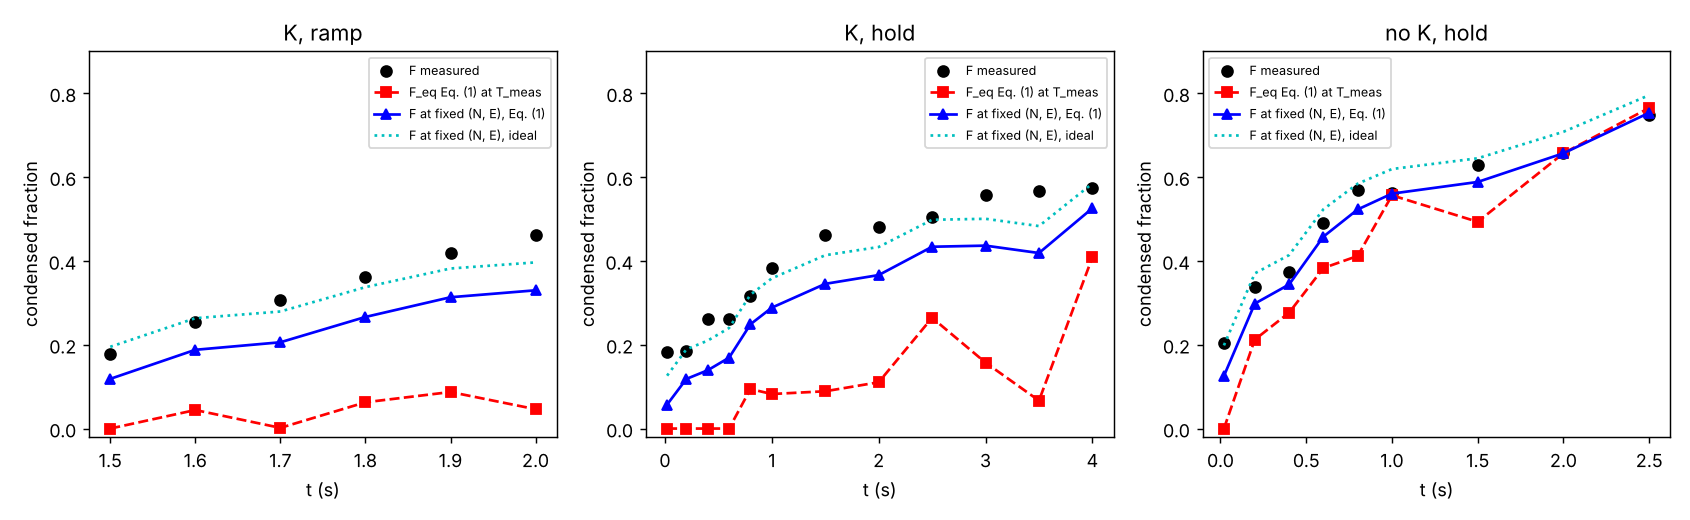
\includegraphics[width=\columnwidth]{../figures/ne_equilibrium.png}
\caption{Measured condensed fraction (circles) of the sample with K during
the last $0.5$~s of the ramp (left), of the sample with K during the hold
(middle) and of the sample without K during the hold (right), compared with
the equilibrium fraction of Eq.~(1) at the measured temperature (squares,
the reference of Ref.~\cite{MelladoMunoz2020}) and with the equilibrium
fraction at the measured atom number and energy (triangles, Eq.~(1);
dotted, ideal gas). Digitized data of Figs.~2 and S2(ii), calibrated trap
frequencies, ideal-gas thermal energy with the fugacity of the measured
thermal cloud [DATA, scripts/15].}
\label{fig:NE}
\end{figure}

Two thirds of the excess of the samples with K, and all of it for the
sample without K, is the reference. The sample without K sits on its
fixed-$(N,E)$ equilibrium to within $0.03$ throughout the hold, with
$T'$ within $-2$ to $+9\%$ of the measured $T$. The samples with K retain a
residual of $0.10\pm0.03$, the same during the ramp and during the hold and
constant over the $4$~s of the hold; equivalently, their measured
temperature lies $7$ to $23\%$ above $T'$. The residual depends on the
reference formula: with the ideal-gas fraction in place of Eq.~(1) it is
$0.02\pm0.03$ (ramp) and $0.03\pm0.03$ (hold), so it is of the size of the
interaction and finite-size shift of $T_c$ in Eq.~(1), which lowers
$F_{\rm eq}$ by $0.05$ to $0.1$ at these numbers. A $3\%$ error in the
measured temperature, the precision of the digitization, moves it between
$0.07$ and $0.12$. The trap frequency does not help: the measured line of
Fig.~S1, $15\%$ below the calibrated one, lowers $T_c$ and raises the
residual to $0.20$, and only a frequency above the calibrated value would
reduce it [DATA].

The question of the relaxation time changes accordingly. The kinetic
models relax the measured states to their fixed-$(N,E)$ equilibrium in
$0.05$~s (ergodic, Sec.~\ref{sec:hold}: $F$ from $0.46$ to $0.40$, the
ideal-gas $F_{N,E}$ of the measured end-of-ramp state) and $0.2$~s
(phase space, deep trap: $F=0.07$ against $F_{N,E}=0.06$ from Eq.~(1) for
the measured initial state of the hold), and the changes involved are
$0.03$ to $0.1$ in $F$. Nothing larger is left to relax. The decay of
$\delta F$ in Fig.~4 is the drift of $N$ and $E$ at fixed trap depth,
through the background loss and the residual evaporation that bring $N$
from $1.57\times10^4$ to $7.2\times10^3$ and $T$ from $111$ to $63$~nK in
$4$~s, which raises $F_{\rm eq}(T)$ toward the measured $F$; its time
constant is that of the loss, not of a thermalization. The scatter of the
digitized $\delta F(t)$ does not allow us to fit the time constant
independently, so we do not quote one; the raw data would.

\section{Discussion}
\label{sec:disc}
The kinetic models reproduce the atom number and the condensed fraction of
the data with and without K, and both reach, within $0.2$~s, the equilibrium
of the measured states at fixed number and energy, which the data sit on to
within $0.03$ (no K) and $0.10\pm0.03$ (K). We have tested the three ways in
which the kinetics could be wrong by a large factor. (i) The collision
integral $I_{12}$: scaling it by $0.5$ or $2$ moves $F(2\,{\rm s})$ with K
from \sensreference{} to \sensCxiiHalf{} and \sensCxiiTwo{}
(Fig.~\ref{fig:sens}) and does not change the temperature. (ii) Heating by
the K atoms through glancing collisions with energy transfer below the trap
depth, added with a rate equal to $\gamma_K$: it raises the temperature at
$t=2$~s by $4\%$ and lowers $F$ from $0.37$ to $0.21$, away from the data.
(iii) The evaporation model: one-direction escape and three-dimensional
truncation, each with its own calibration, give the same temperature with
and without K and $F(2\,{\rm s})$ with K within $0.06$ of each other.
Dropping the ergodic approximation (Secs.~\ref{sec:aniso} and
\ref{sec:phasespace}) changes the depletion time of an undersaturated state
from $0.05$ to $0.2$~s and leaves the fixed point unchanged.

Two discrepancies remain, and they are of a different kind from the one
the two-mode model was built for. The first is the residual $0.10\pm0.03$ of
the samples with K, which is constant over the $4$~s of the hold and
therefore not kinetic: anything that relaxes by collisions does so in
$0.05$ to $0.2$~s in both models. It is equivalent to a measured
temperature $7$ to $23\%$ above the temperature of the fixed-$(N,E)$
equilibrium, while the sample without K shows no such offset. Three
explanations have the right size and sign. (a) The interaction shift in
Eq.~(1), since the residual vanishes within the scatter for the ideal-gas
reference; the shift itself is not in question, but its evaluation with a
Gaussian-fit temperature and a Thomas-Fermi condensate number at $N_0$ of a
few $10^3$ is. (b) A systematic in the temperature of the K sequences,
of order $10\%$, which the raw images can test: if the vertical width of
the thermal cloud gives a lower temperature than the horizontal one, the
offset is in the fit. (c) A non-thermal component bound in the arms of the
crossed trap: an atom that leaves the crossing region along a beam stays
radially bound and returns after half an axial period, $2\pi(mz_R^2/2U_b)^{1/2}$,
which is $2$ to $4$~s for a beam depth of $0.5\,\mu$K and
Rayleigh ranges of $3.6$ and $6$~mm ($\lambda=1064$~nm [CONFIRM?]), and
such atoms raise the horizontal Gaussian width without taking part in the
exchange with the condensate. The arms are the only place where bound
atoms with energies above the trap depth can exist, and the quadrupole
field of the MOT tilts them by about $10\,\mu$K per mm per $0.1\,g$, which
would make the K and no-K sequences differ if the field is on in only one
of them [CONFIRM?]. (a) and (b) are decided by refitting the existing
images; (c) by the dependence of the residual on the beam power during the
hold, which sets the axial period as $P^{-1/2}$.

The second discrepancy is on the model side. With K, the models arrive at
the measured $N$ and $F$ with a thermal cloud that holds $20$ to $25\%$ less
energy than the measured state at its fixed-$(N,E)$ equilibrium ($51$~nK
against $T'=65$~nK at the end of the ramp in the ergodic model; a Bose
temperature of about $60$~nK against $T'=70$~nK at $2$~s of the hold in the
phase-space model, once its kinetic temperature is corrected for the $0.9$
factor of a saturated cloud and the $10$ to $15\%$ low-energy bias of the
test-particle cloud). The models remove too much energy with K, or the K
atoms deposit energy that the uniform loss does not describe. The $t^2$ time
dependence of the K-induced loss, against the measured K density, points the
same way: the Rb-K collisions do more to the Rb gas than removing atoms at
the rate of Fig.~1(b), and the energy balance of that interaction is the
open input of the models [CONFIRM?].

\section{Conclusion}
We have solved the quantum-kinetic equations for the dissipative
distillation experiment with the thermal cloud evolving self-consistently,
in the ergodic approximation and in phase space with the real trap
geometry. With one calibration on the data without K and the measured loss,
the ergodic model gives the atom number and the condensed fraction of the
distillation data to better than $0.05$ in $F$; the phase-space model
reproduces the hold phase from the measured initial states with the trap
depth as its only parameter. The main result is a change of reference. The
measured states lie within $0.03$ (no K) and $0.10\pm0.03$ (K) of the
equilibrium at their own atom number and energy, which is the only
equilibrium a trapped gas without a bath can reach; both models reach it in
$0.05$ to $0.2$~s. Two thirds of the excess fraction reported relative to
the constant-temperature curve, and the whole of it for the sample without
K, is the difference between the two references, and the $3.9$~s decay of
that excess is the drift of $N$ and $E$ by loss and residual evaporation at
fixed trap depth, not a thermalization time. The limitation of this
statement is the residual $0.10\pm0.03$ of the samples with K, which is
constant in time, of the size of the interaction shift in the equilibrium
formula, and equivalent to a $10$ to $20\%$ temperature offset. The next
step is a refit of the existing images, with the temperature from the
vertical width and a two-component or Bose profile for the thermal part,
which decides whether the residual is in the fit, in the formula, or in a
population bound in the arms of the trap.
